% !TEX root = Calli.tex

\section{Programmstruktur / Methodik}
\label{sec:Programmstruktur}

Zum Lösen der Aufgabe wird die Programmiersprache \emph{Python 2.7} verwendet. In Form der Open-Source Library \emph{OpenCV} steht dazu eine leistungsstarke Bibliothek zur Bildverarbeitung zur Verfügung.
OpenCV selbst ist in C++ geschrieben, bietet jedoch entsprechende Python-Bindings an.


\subsection{Initialisierung}

Favorisiert wird eine extern angeschlossene Webcam angesprochen. Findet die Software keine Kamera, so greift sie auf die interne Kamera des Laptops zu. 

\lstset{language=Python}
\begin{lstlisting}[]
# try to use an external webcam if possible
cap = cv2.VideoCapture(1)
if not cap.isOpened():
    # use the internal cam
    cap = cv2.VideoCapture(0)
\end{lstlisting}

\textbf{HSV-Raum}

Um die einzelnen Früchte sicher detektieren zu können, wird zuerst das Ausgangsbild in den HSV-Raum übertragen. Jede Farbe wird mit Hilfe des Farbwinkel (hue) auf dem Farbkreis (z.B. 0$^\circ$/360$^\circ$  für rot), der Farbsättigung (saturation) in Prozent (z.B. 0\% Neutralgrau) und des Hellwertes (value) in Prozent (z.B.100\% volle Helligkeit) definiert.
\begin{figure}[H]
    \centering
    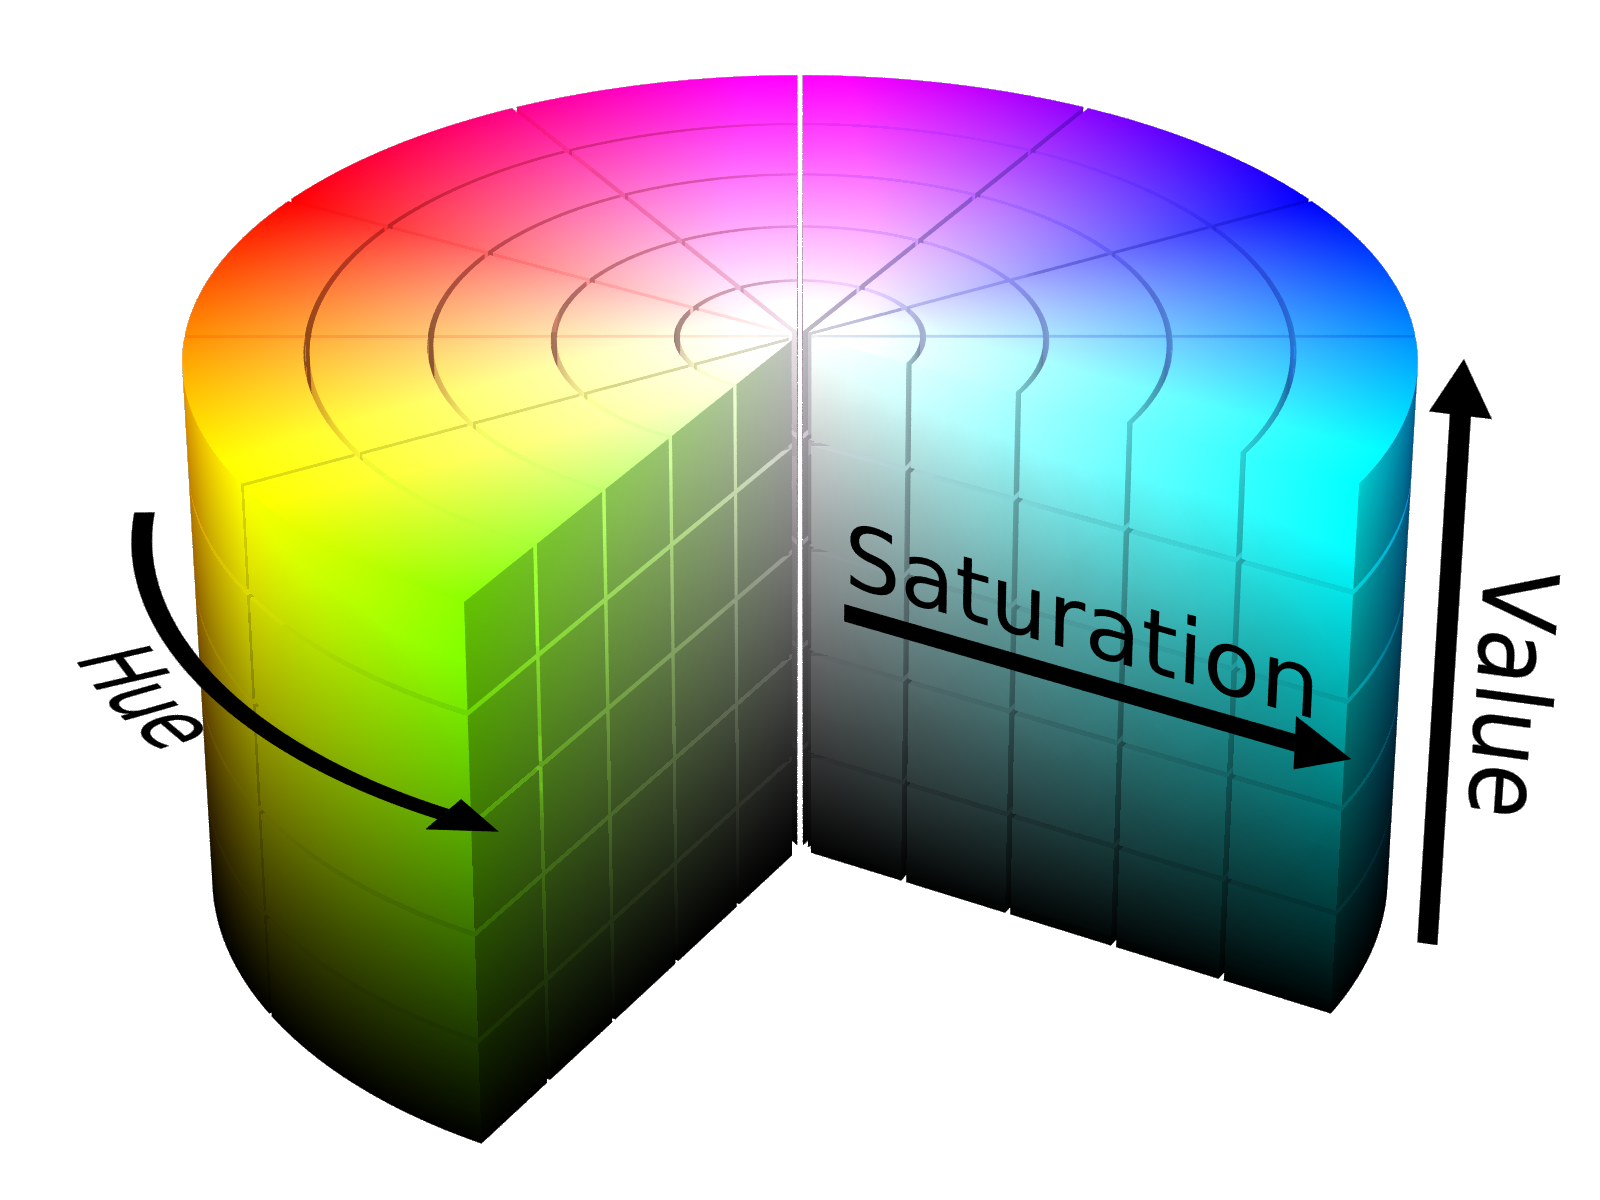
\includegraphics[width=0.4\textwidth]{Abbildungen/HSV_color}
    \caption[HSV]{HSV-Farbraum}
    \label{fig:HSV-Farbraum}
\end{figure}
\lstset{language=Python}
\begin{lstlisting}[]
    # read the frames
    _, frame = cap.read()
    # transform frame to HSV
    hsv = cv2.cvtColor(frame, cv2.COLOR_BGR2HSV)
\end{lstlisting}
In OpenCV wird der Farbwinkel mit 8Bit im Bereich von 0 bis 179, die Farbsättigung mit vollen 8Bit von 0 bis 255 und die Helligkeit mit vollen 8Bit von 0 bis 255 dargestellt.
Für die Farben der Früchte des Halli Galli Spiels ist der HSV-Raum fest definiert. Die Bereiche zur Filterung werden entsprechend darum festgelegt. 

\begin{itemize}
    \item Erdbeere - rot - HSV(3, 73\%, 70\%)
    \item Pflaume - lila - HSV(329, 68\%, 45\%)
    \item Limone - hellgrün - HSV(93, 64\%, 57\%)
    \item Banane - gelb - HSV(53, 72\%, 69\%)
\end{itemize}

Minimum - und Maximumwert für die Farbbereiche der Früchte können zur Kalibrierung über Schieberegler eingestellt werden. Abhängig von der Beleuchtung und der verwendeten Kamera variieren diese, sodass eine Anpassung zum Beginn des Prozesses sinnvoll ist. 

\subsubsection{Schwellwertverfahren}

Mit Hilfe einer Segmentierung über ein Schwellwertverfahrens wird das Ausgangsbild für jede Fruchtsorte gefiltert und jeweils ein Binärbild erstellt.
Da bei den Erdbeeren die Farbe Rot an den Grenzen des Farbwinkelwertes liegt, werden hier zwei Schwellwertoperationen durchgeführt und diese anschließen bitweise mit ODER zu einem verknüpft werden.
\lstset{language=Python}
\begin{lstlisting}[]
    # use Threshold for Strawberries
    thresh1_low = cv2.inRange(
        hsv,
        np.array((0, lower_s_s, lower_v_s)),
        np.array((0 + h_s, upper_s_s, upper_v_s)))
    thresh1_high = cv2.inRange(
        hsv,
        np.array((180 - h_s, lower_s_s, lower_v_s)),
        np.array((180, upper_s_s, upper_v_s)))

    thresh1 = cv2.bitwise_or(thresh1_low, thresh1_high)
\end{lstlisting}

\subsubsection{Filter}

Für jede Frucht wird das Ausgangsbild mit einem Closing - Operator und einem Opening - Operator gefiltert. Während durch das Closing dunkle Störungen im Bild unterdrückt werden, vermindert das Opening lokale Störungen durch helle Bildpunkte.  \\
\lstset{language=Python}
\begin{lstlisting}[]
    # Opening
    thresh3 = cv2.morphologyEx(thresh3, cv2.MORPH_OPEN, kernel)
    # Closing
    thresh3 = cv2.morphologyEx(thresh3, cv2.MORPH_CLOSE, kernel)
\end{lstlisting}

\textbf{Konturerkennung}
%beschreibung der Konturerkennung vllt. an Hand der Skrips

\lstset{language=Python}
\begin{lstlisting}[]
    strawberry_contours, strawberry_hierarchy = cv2.findContours(
        thresh1,
        cv2.RETR_LIST,
        cv2.CHAIN_APPROX_SIMPLE)
\end{lstlisting}

\subsection{Formsegmentierung}

Wenn alle Pixel in den Farben der Früchte entdeckt und segmentiert sind, ist es notwendig die Form der gefundenen Segmente zu untersuchen. Dazu werden für jede Frucht verschiedene geometrische Verhältnisse betrachtet.
\begin{itemize}
    \item Größe der Fläche
    \item Seitenverhältnis des kleinst - möglich umgebenden Rechteckes
    \item Verhältnis Größe der Fläche zu Größe des kleinst - möglich umgebenden Rechteckes
\end{itemize}
Im Fall der Bananen muss zusätzlich die Ausrichtung des umschließenden Rechtecks überprüft werden, um den zutreffenden Bereich zu verkleinern. 
Zur Justierung der Parameter werden WErte an den Konturen ausgegeben.
\lstset{language=Python}
\begin{lstlisting}[]
    # Find Bananas
    bananas = [ ]
    for cnt in banana_contours:

        banana_area = cv2.contourArea(cnt)
        (x_c, y_c), radius = cv2.minEnclosingCircle(cnt)

        center = int(x_c), int(y_c)
        radius = int(radius)
        rect = cv2.minAreaRect(cnt)
        pos, size, theta = rect
        box = cv2.cv.BoxPoints(rect)
        box = np.int0(box)
        x, y = pos
        w, h = size

        if 300 < banana_area < 900:
            if h < w:
                w, h = h, w
            if 2.0 < h / w < 3.9:
                area_rate = w * h / banana_area  # 1.7
                if 1.2 < area_rate < 2.9:
                    bananas.append(cnt)
                    # draw_str(
                    #   frame,
                    #   (int(x)+radius, int(y)),
                    #   str(h/w))
                    # draw_str(
                    #   frame,
                    #   (int(x)+radius, int(y)+24),
                    #   str(banana_area))
                    # draw_str(
                    #   frame,
                    #   (int(x)+radius, int(y)+12),
                    #   str(area_rate))
                    # cv2.drawContours(frame,[box],0,(0,255,0),2)
\end{lstlisting}
\begin{figure}[H]
    \centering
    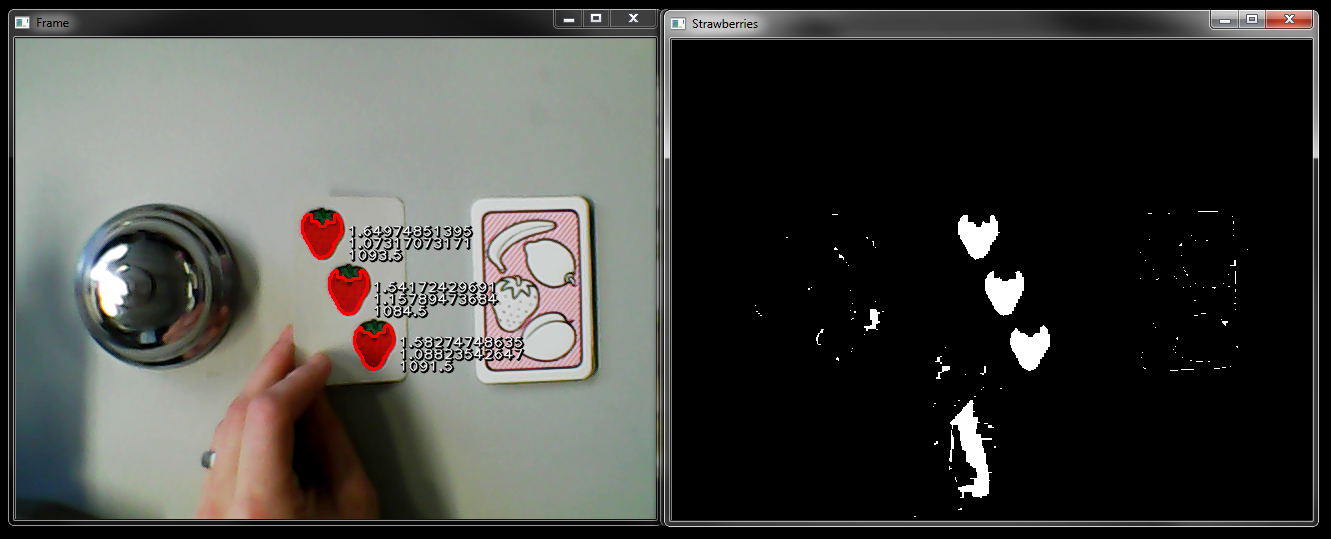
\includegraphics[width=\textwidth]{Abbildungen/Erdbeeren03}
    \caption[]{Erkannte Erdbeeren mit ausgegebenen Werten der Konturen}
    \label{fig:Erdbeeren03}
\end{figure}
\begin{figure}[H]
    \centering
    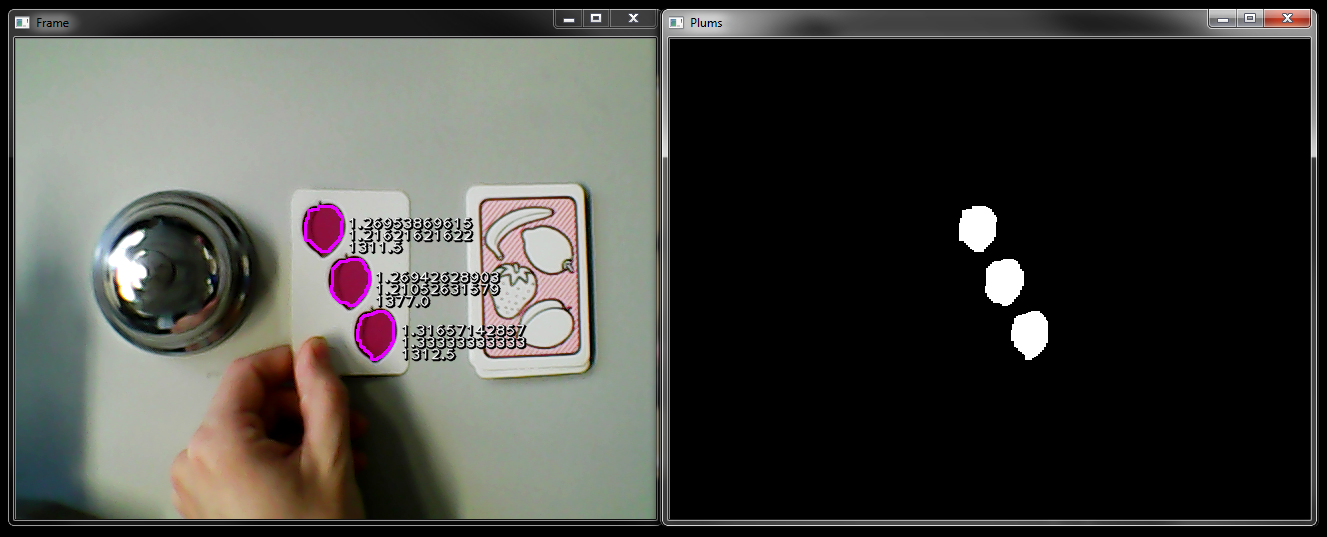
\includegraphics[width=\textwidth]{Abbildungen/Pflaumen03}
    \caption[]{Erkannte Pflaumen mit ausgegebenen Werten der Konturen}
    \label{fig:Pflaumen03}
\end{figure}
\begin{figure}[H]
    \centering
    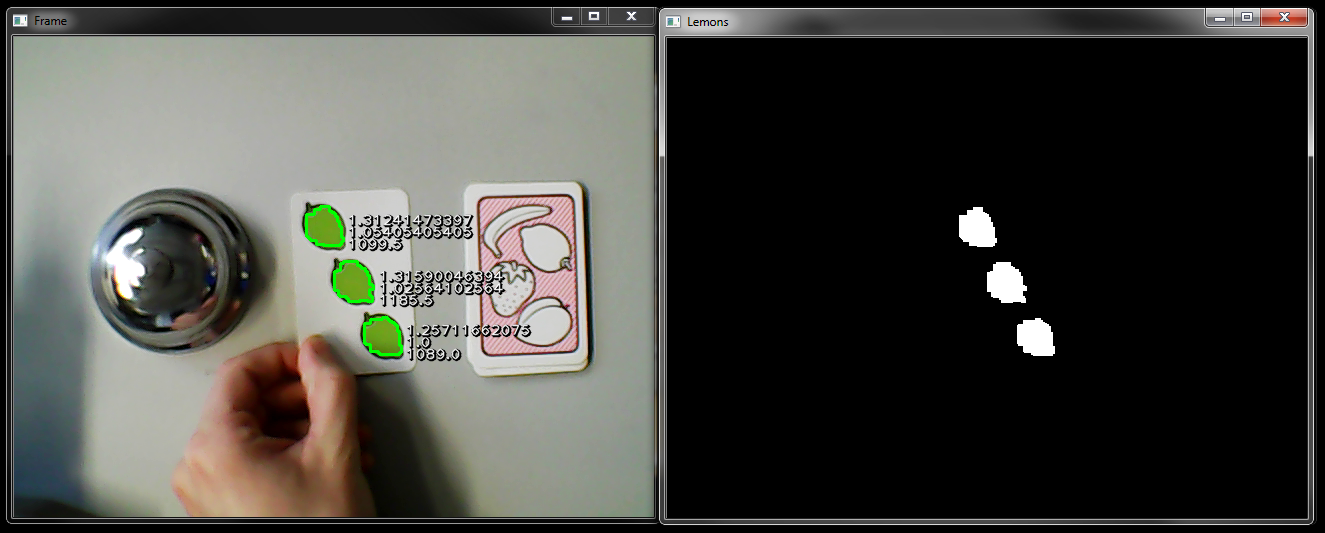
\includegraphics[width=\textwidth]{Abbildungen/Limetten03}
    \caption[]{Erkannte Limonen mit ausgegebenen Werten der Konturen}
    \label{fig:Limetten03}
\end{figure}
\begin{figure}[H]
    \centering
    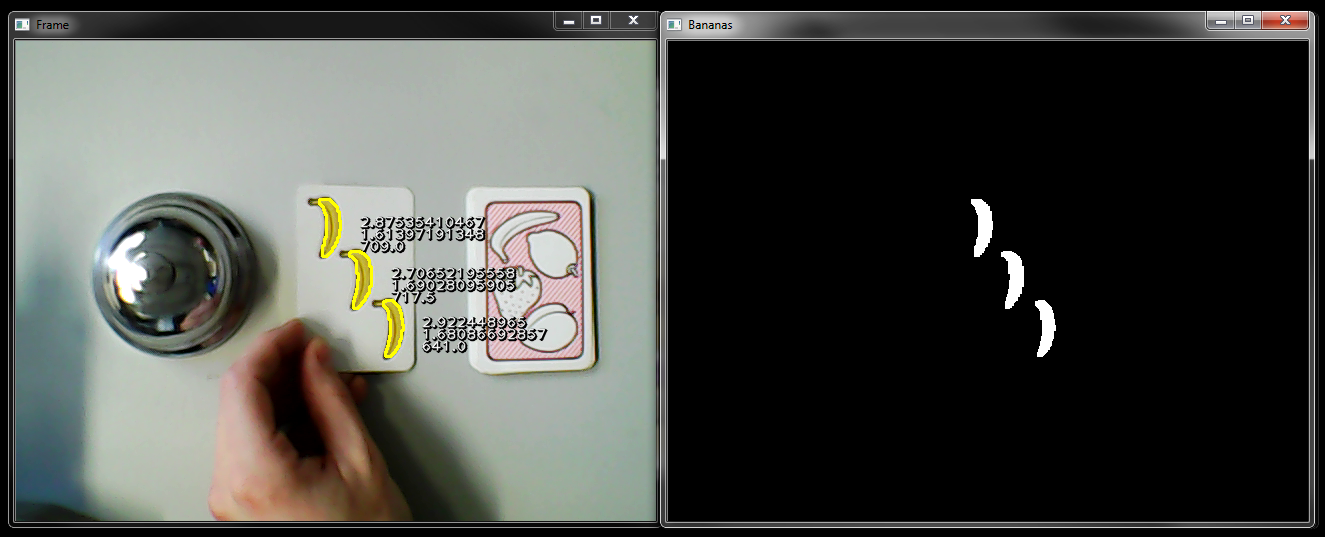
\includegraphics[width=\textwidth]{Abbildungen/Bananen03}
    \caption[]{Erkannte Bananen mit ausgegebenen Werten der Konturen}
    \label{fig:Bananen03}
\end{figure}

\subsection{Visualisierung}
\lstset{language=Python}
\begin{lstlisting}[]
    cv2.namedWindow('Frame')
    cv2.drawContours(frame, strawberries, -1, (0, 0, 255), 2)
    cv2.drawContours(frame, plums, -1, (255, 0, 230), 2)
    cv2.drawContours(frame, lemons, -1, (0, 255, 0), 2)
    cv2.drawContours(frame, bananas, -1, (0, 255, 255), 2)

    if len(strawberries) == 5:
        # print "Strawberries!"
        draw_str(frame, (20, 20), "Strawberries!!!!!")
    if len(plums) == 5:
        # print "Plums!"
        draw_str(frame, (20, 40), "Plums!!!!!")
    if len(lemons) == 5:
        # print "Lemons!"
        draw_str(frame, (20, 60), "Lemons!!!!!")
    if len(bananas) == 5:
        # print "Bananas!"
        draw_str(frame, (20, 80), "Bananas!!!!!")

    cv2.imshow('Frame', frame)
\end{lstlisting}

Die gefunden Früchte werden gezählt. Wenn genau fünf Früchte von einer Sorte gefunden werden, signalisiert ein Schriftzug auf dem Bildschirm, dass die Glocke geläutet werden muss. Auf die Glocke fertig - los!

